\documentclass[a4paper,12pt]{article}
\usepackage[utf8]{inputenc}
\usepackage{amsmath, amssymb}
\usepackage{graphicx}
\usepackage{geometry}
\geometry{margin=2.5cm}

\title{Planificación Óptima de Horarios de Apagón por Bloques: Modelo y Algoritmo}
\author{Adrián Alejandro Souto Morales C312 \\ Gabriel Herrera Carrazana C312}
\date{\today}

\begin{document}

\maketitle

\begin{abstract}
Este documento describe el modelo matemático y el algoritmo de optimización implementados en el proyecto \textbf{UNE Optimization} para la asignación eficiente y equitativa de cortes de energía eléctrica entre bloques geográficos. Se detalla la lógica de cálculo de demanda, generación y déficit, así como la generación del horario óptimo de apagón por bloques, junto a la metodología de resolución basada en programación matemática y optimización numérica.
\end{abstract}

\section{Introducción}
El proyecto \textbf{UNE Optimization} permite planificar los horarios de corte de energía a nivel provincial, considerando la demanda eléctrica, la generación disponible y el déficit resultante. El sistema guía al usuario desde la configuración de parámetros hasta la visualización de los horarios óptimos de apagón por bloques.

\section{Cálculo de la demanda, generación y déficit}
El usuario puede configurar el consumo promedio por provincia y la generación disponible por termoeléctrica. A partir de estos datos, el sistema calcula el déficit energético y distribuye la cantidad de horas de corte necesarias para cada provincia, de modo que el total de energía no suministrada compense el déficit.

\begin{itemize}
    \item \textbf{Demanda por provincia} ($D_i$): configurada por el usuario o por defecto.
    \item \textbf{Generación total} ($G$): suma de la capacidad diaria de todas las termoeléctricas.
    \item \textbf{Asignación óptima} ($A_i$): se obtiene resolviendo una optimización que minimiza el error cuadrático entre la demanda y la energía asignada a cada provincia, normalizado por el consumo horario:
    \begin{equation}
        \min_{A_i} \sum_{i=1}^{N} \frac{(D_i - A_i)^2}{D_i/24}
    \end{equation}
    \item \textbf{Restricciones:}
    \begin{itemize}
        \item $\sum_{i=1}^{N} A_i \leq G$
        \item $A_i \geq 0$
        \item Para La Habana: $A_{Habana} \geq 0.05 \cdot D_{Habana}$
    \end{itemize}
    \item \textbf{Déficit por provincia} ($\Delta_i$):
    \begin{equation}
        \Delta_i = D_i - A_i
    \end{equation}
    \item \textbf{Horas de corte por provincia} ($H_i$):
    \begin{equation}
        H_i = \frac{\Delta_i}{D_i/24}
    \end{equation}
\end{itemize}

\section{Generación del horario óptimo de apagón por bloques}
Una vez calculadas las horas de corte necesarias para cada provincia, el sistema permite definir la cantidad de bloques (zonas) y genera, para cada bloque, una matriz $24 \times 7$ (horas x días) con valores binarios: 1 si hay corte en la hora $i$ del día $j$, 0 si no. Los cortes diarios son consecutivos y de duración exacta, minimizando la superposición entre bloques y distribuyendo equitativamente los cortes a lo largo del día.

\begin{itemize}
    \item Para cada bloque $b$ y día $d$, se definen variables $s_{b,d}$ (inicio) y $e_{b,d}$ (fin), con $e_{b,d} - s_{b,d} = h_c$.
    \item Se construye una matriz binaria $M^{(b)}$ de $24 \times 7$, marcando con 1 las horas entre $s_{b,d}$ y $e_{b,d}$.
    \item La matriz de solapamiento es $O_{h,d} = \sum_{b=1}^B M_{h,d}^{(b)}$.
\end{itemize}

La función objetivo a minimizar es:
\begin{equation}
J = \sum_{h=1}^{24} \sum_{d=1}^7 O_{h,d} + \frac{1}{2} \sum_{h=1}^{24} \sum_{d=1}^7 [O_{h,d} > 1] (O_{h,d} - 1)
\end{equation}
Donde el primer término promueve la equidad horaria y el segundo penaliza la superposición.

\section{Estrategia de Optimización}
Se utiliza \texttt{scipy.optimize.minimize} (SLSQP) para encontrar los horarios de corte óptimos:
\begin{itemize}
    \item Las variables de decisión son los horarios de inicio y fin de corte para cada bloque y día, restringidos a ser consecutivos y de duración exacta.
    \item Se inicializan aleatoriamente los horarios válidos.
    \item Se calcula la función objetivo y se ajustan los horarios para minimizarla.
\end{itemize}

\section{Tecnologías y Frameworks Utilizados}
La implementación de \textbf{UNE Optimization} se apoya en tecnologías modernas para el desarrollo eficiente y la visualización interactiva:
\begin{itemize}
    \item \textbf{Python}: Lenguaje principal para el backend y la lógica de optimización.
    \item \textbf{scipy.optimize} y \textbf{numpy}: Para la optimización numérica y manipulación de matrices.
    \item \textbf{matplotlib}: Para la generación de gráficos de los horarios de corte.
    \item \textbf{FastAPI} (o similar): Framework para exponer la API REST del backend.
    \item \textbf{React} y \textbf{TypeScript}: Para el desarrollo del frontend y la visualización interactiva de los resultados.
\end{itemize}

\section{Interfaz de Usuario y Flujo de Interacción}
El frontend de \textbf{UNE Optimization} está diseñado para guiar al usuario a través de todo el proceso de planificación y análisis. Las principales secciones y opciones configurables son:
\begin{itemize}
    \item \textbf{Pantalla de inicio}: Presenta una visión general del sistema y acceso a las funcionalidades principales.
    \item \textbf{Configuración de parámetros}: Permite al usuario ingresar el consumo promedio por provincia y la generación disponible por cada termoeléctrica.
    \item \textbf{Selección de provincia}: El usuario puede seleccionar la provincia para la cual desea planificar los cortes.
    \item \textbf{Configuración de bloques}: Permite definir la cantidad de bloques (zonas) en la provincia seleccionada.
    \item \textbf{Planificación de cortes}: El sistema calcula automáticamente el déficit energético y la cantidad de horas de corte necesarias para cada provincia, mostrando la asignación de MW y horas de corte por bloque.
    \item \textbf{Visualización de resultados}: Se presentan gráficos interactivos que muestran la relación entre demanda y MW asignados, así como los horarios de corte por bloque y día.
    \item \textbf{Opciones de exportación}: El usuario puede descargar los resultados y gráficos generados para su análisis o presentación.
\end{itemize}
El flujo de interacción es intuitivo: el usuario configura los parámetros iniciales, selecciona la provincia y bloques, revisa la planificación sugerida y analiza los resultados visuales para tomar decisiones informadas.

\section{Referencias}
\begin{itemize}
    \item \texttt{scipy.optimize.minimize (SLSQP)}: https://docs.scipy.org/doc/scipy/reference/generated/scipy.optimize.minimize.html
    \item Programación matemática y penalizaciones en optimización restringida.
\end{itemize}

\appendix
\section*{Anexo: Imágenes de Resultados}
A continuación se presentan imágenes de ejemplo generadas por el sistema:

\begin{figure}[h!]
    \centering
    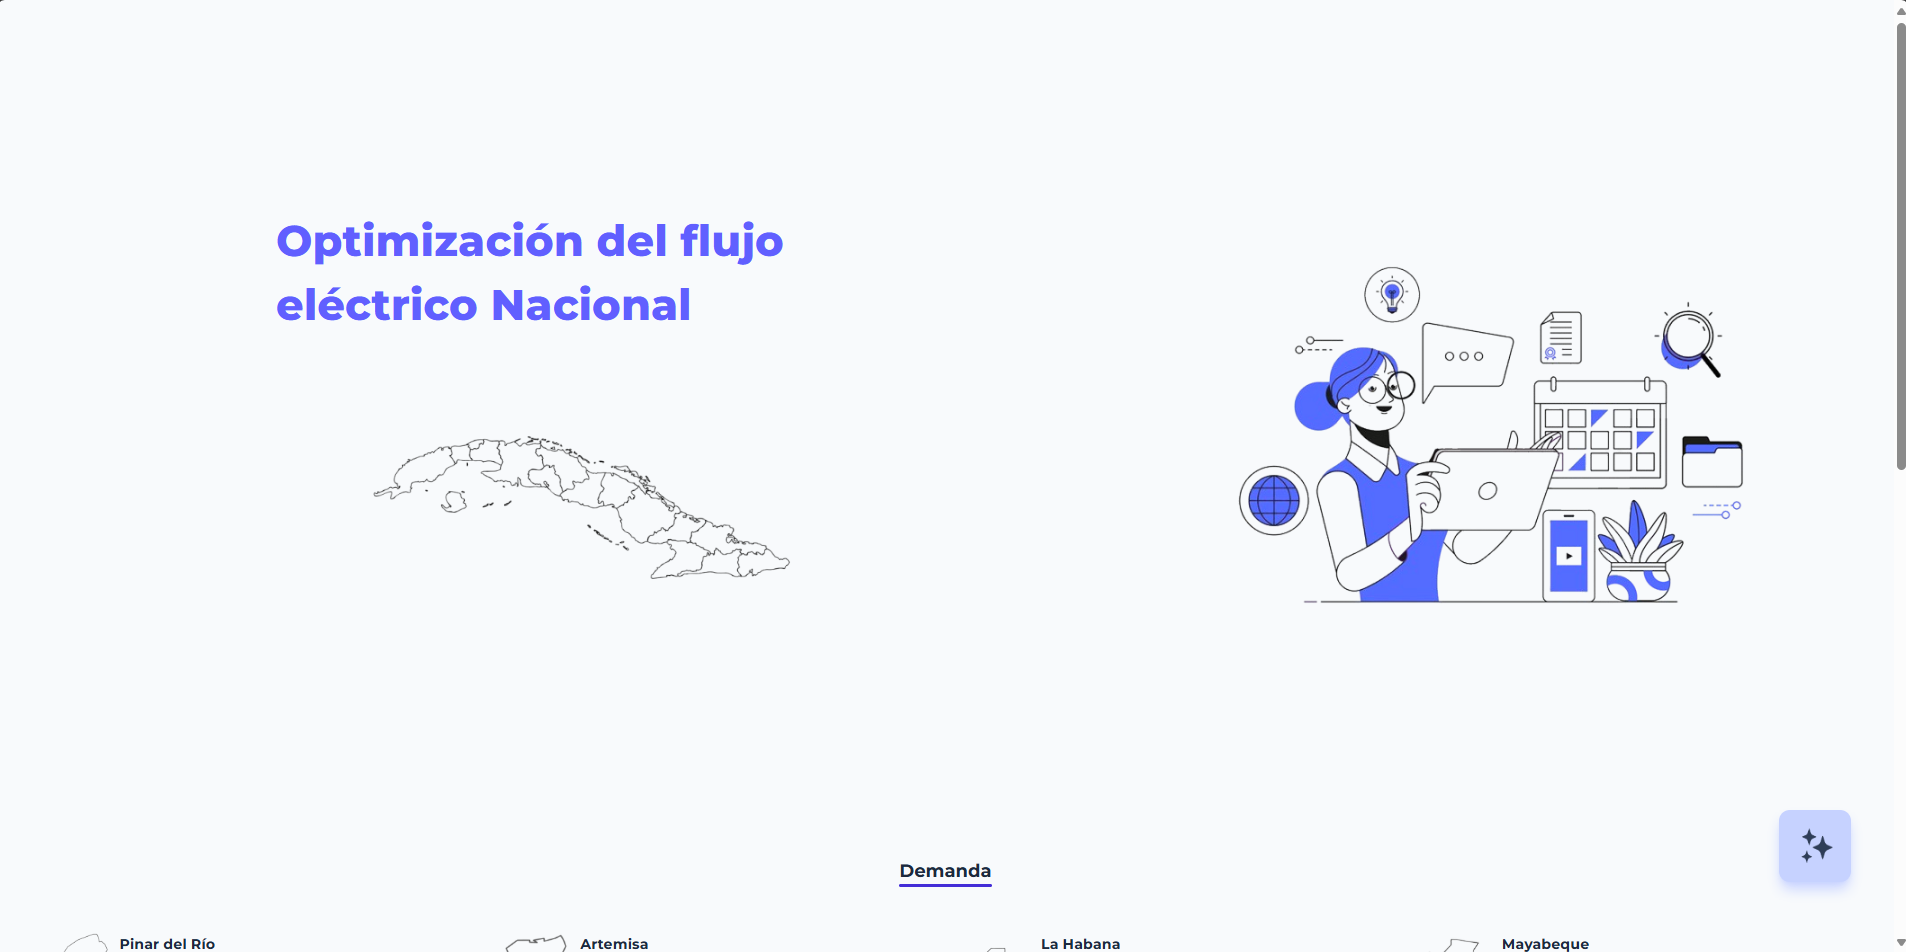
\includegraphics[width=0.8\textwidth]{anexos/1.png}
    \caption{Pantalla de inicio}
\end{figure}

\begin{figure}[h!]
    \centering
    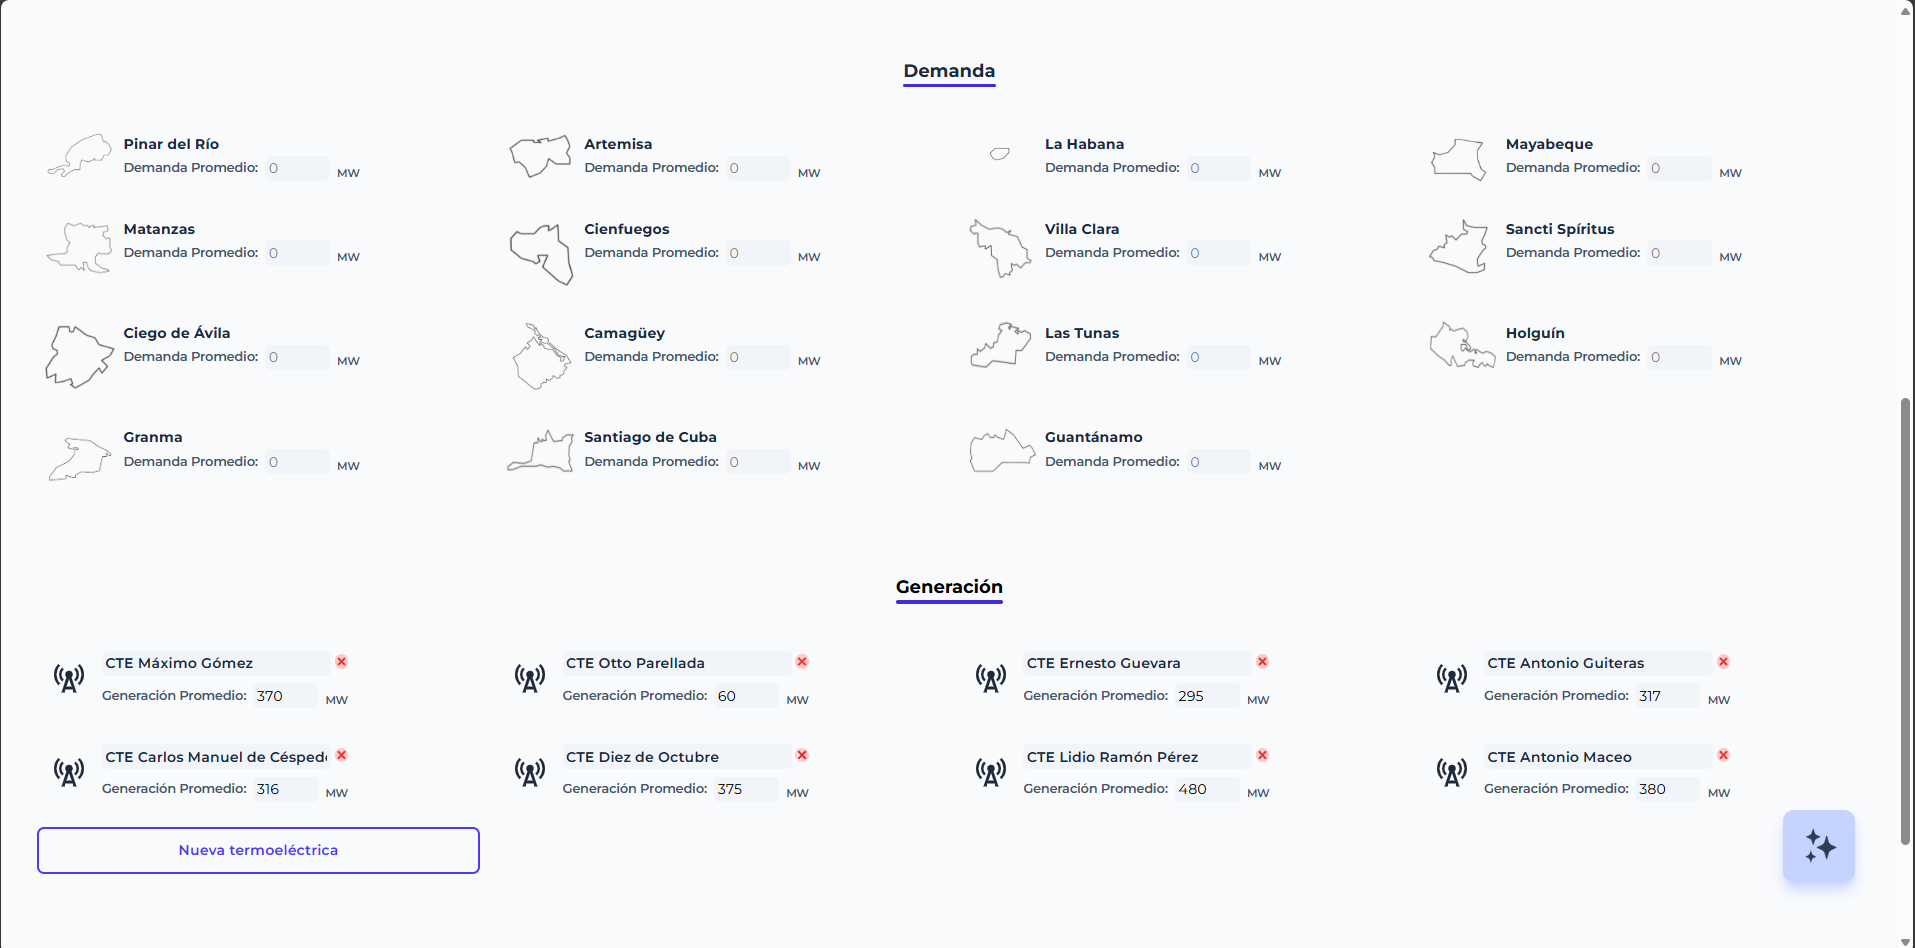
\includegraphics[width=0.8\textwidth]{anexos/2.png}
    \caption{Configuración de consumo promedio por provincias y generación por termoeléctrica}
\end{figure}

\begin{figure}[h!]
    \centering
    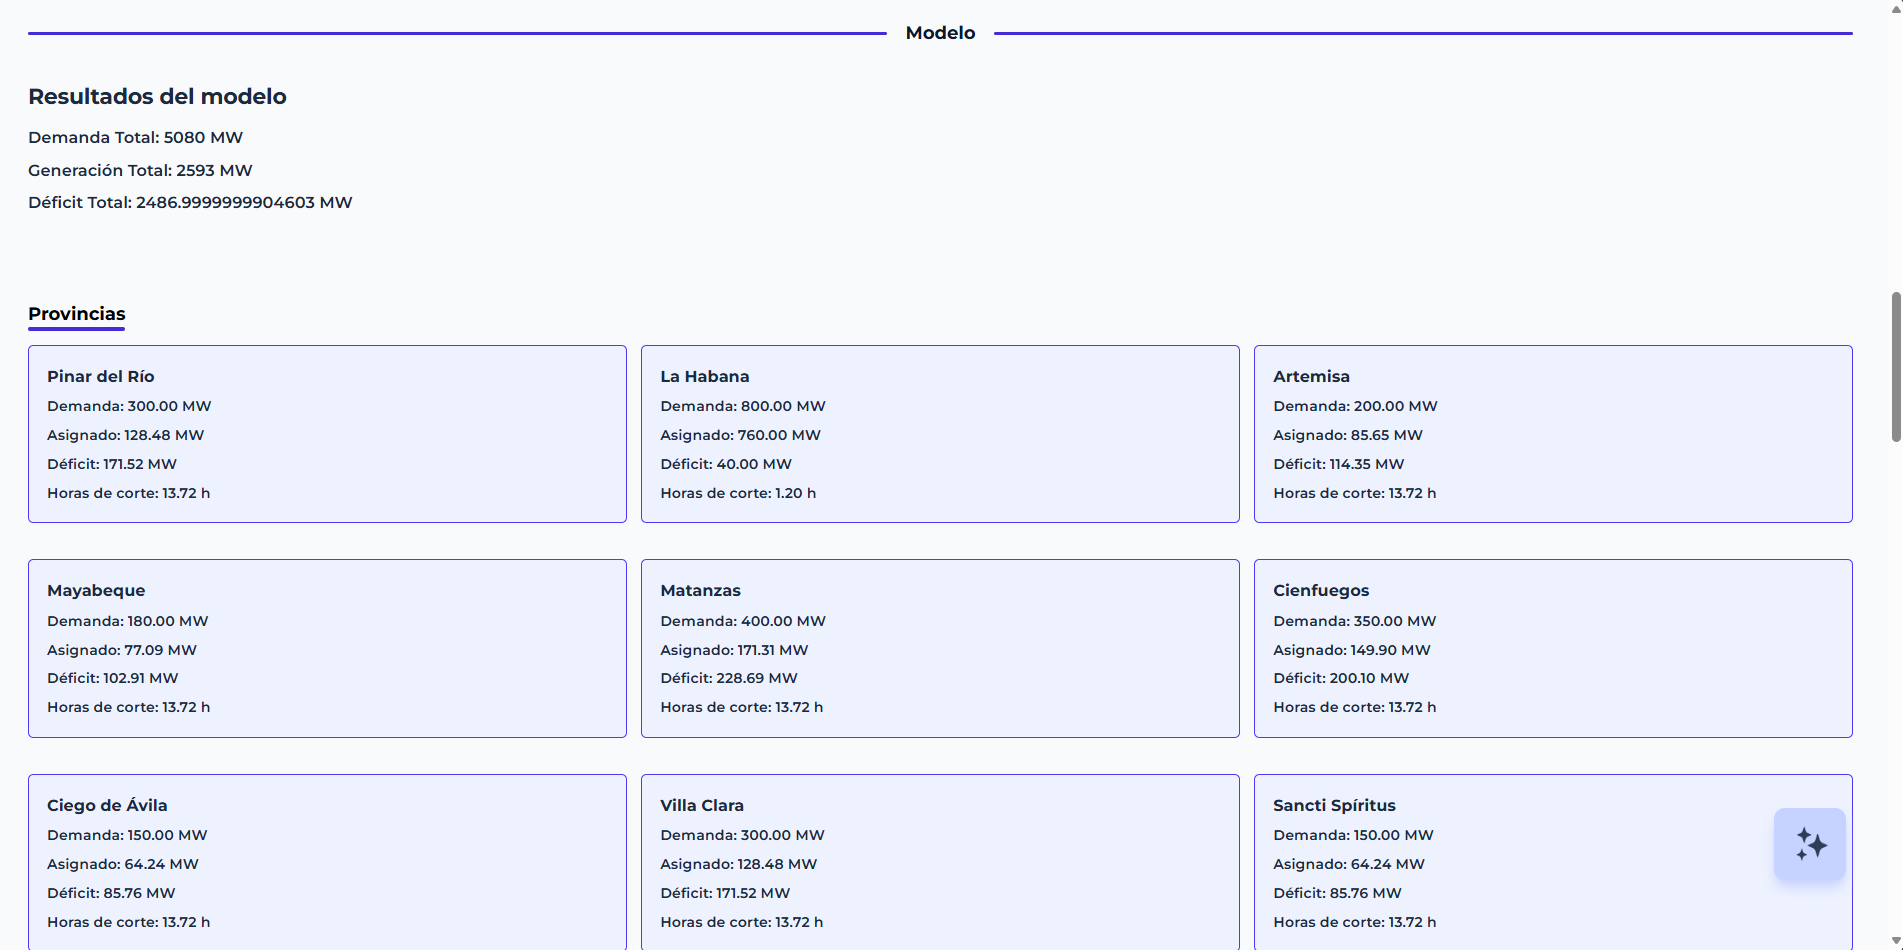
\includegraphics[width=0.8\textwidth]{anexos/3.png}
    \caption{Cálculo de demanda por provincia, así como planificación de cantidad de horas de corte y MW asignados a cada una}
\end{figure}

\begin{figure}[h!]
    \centering
    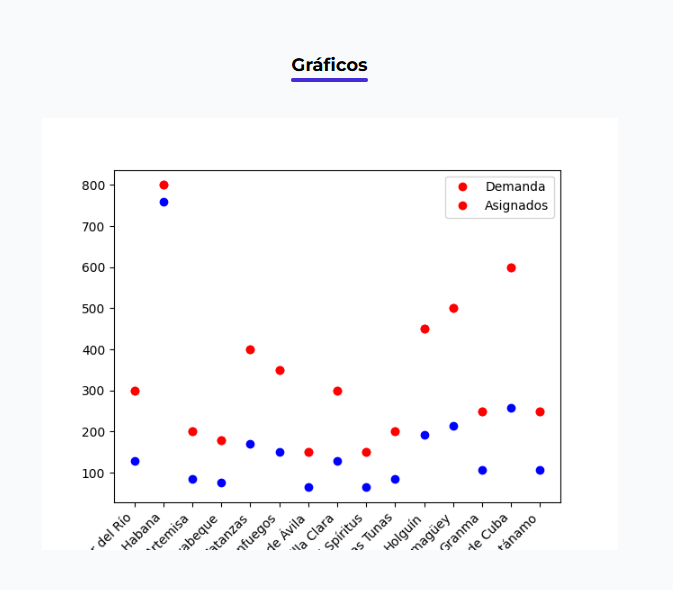
\includegraphics[width=0.8\textwidth]{anexos/4.png}
    \caption{Visualización de relación entre la demanda y MW asignados por provincia}
\end{figure}

\begin{figure}[h!]
    \centering
    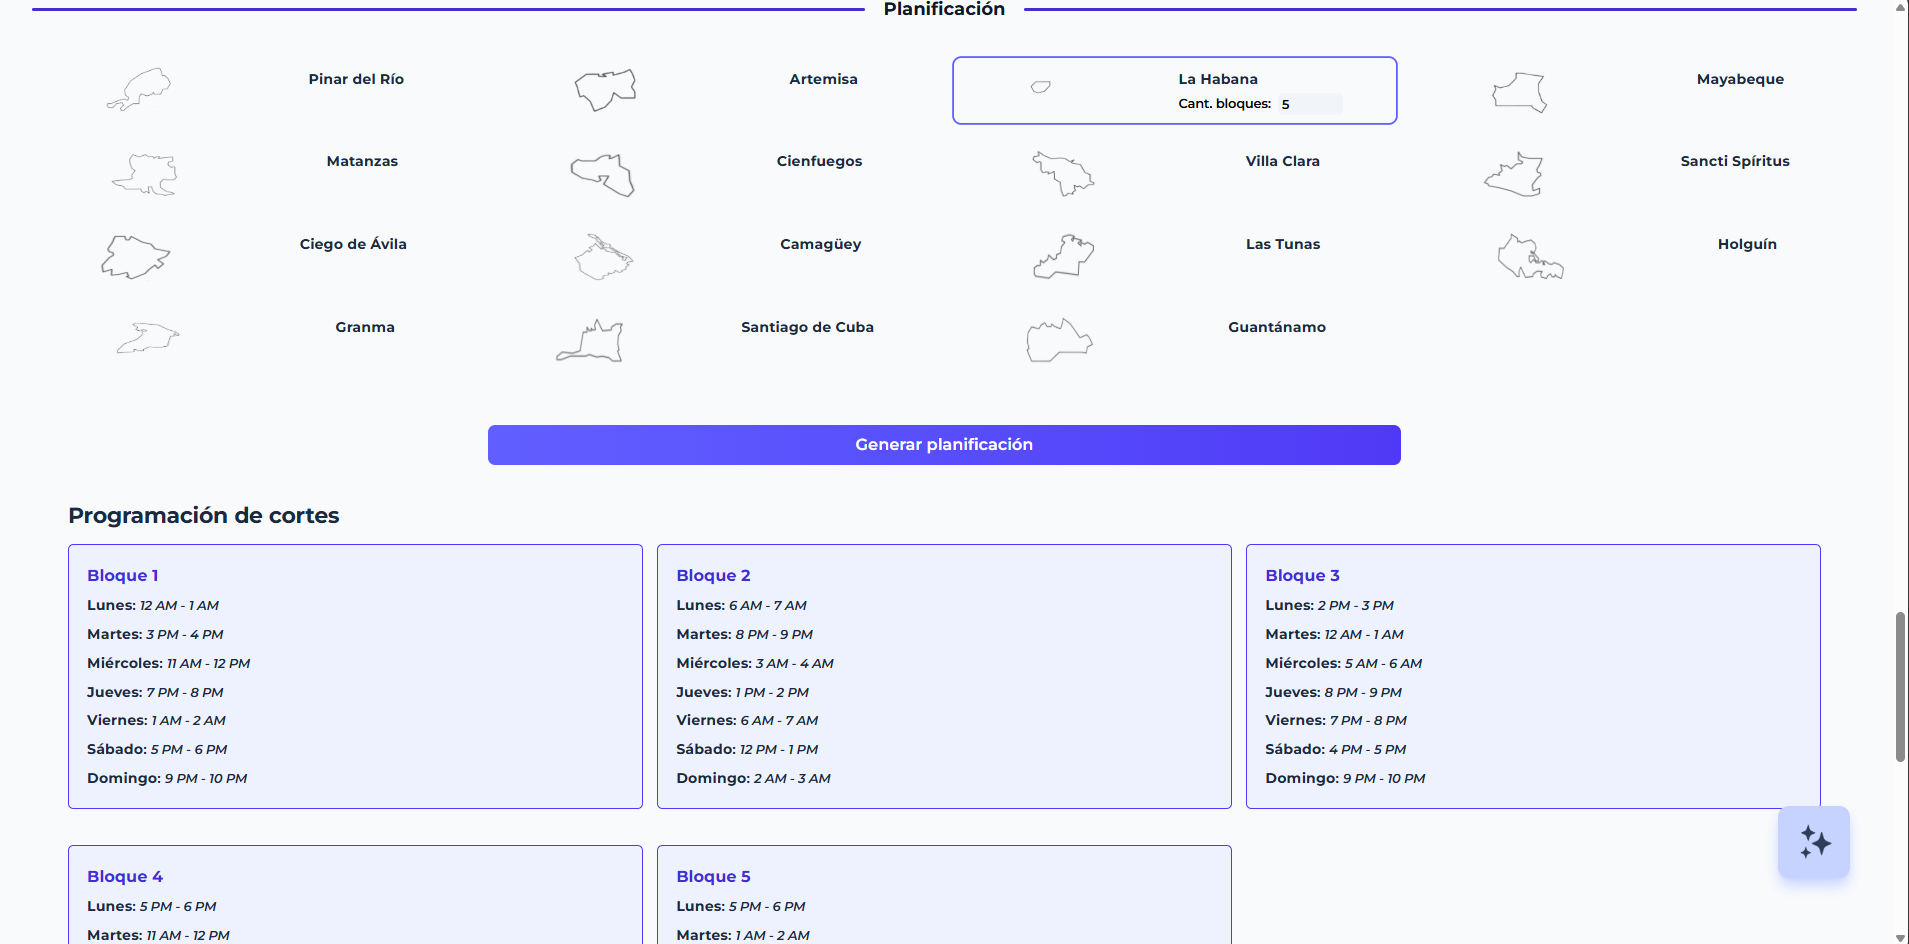
\includegraphics[width=0.8\textwidth]{anexos/5.png}
    \caption{Visualización de horarios de corte por bloque}
\end{figure}

\begin{figure}[h!]
    \centering
    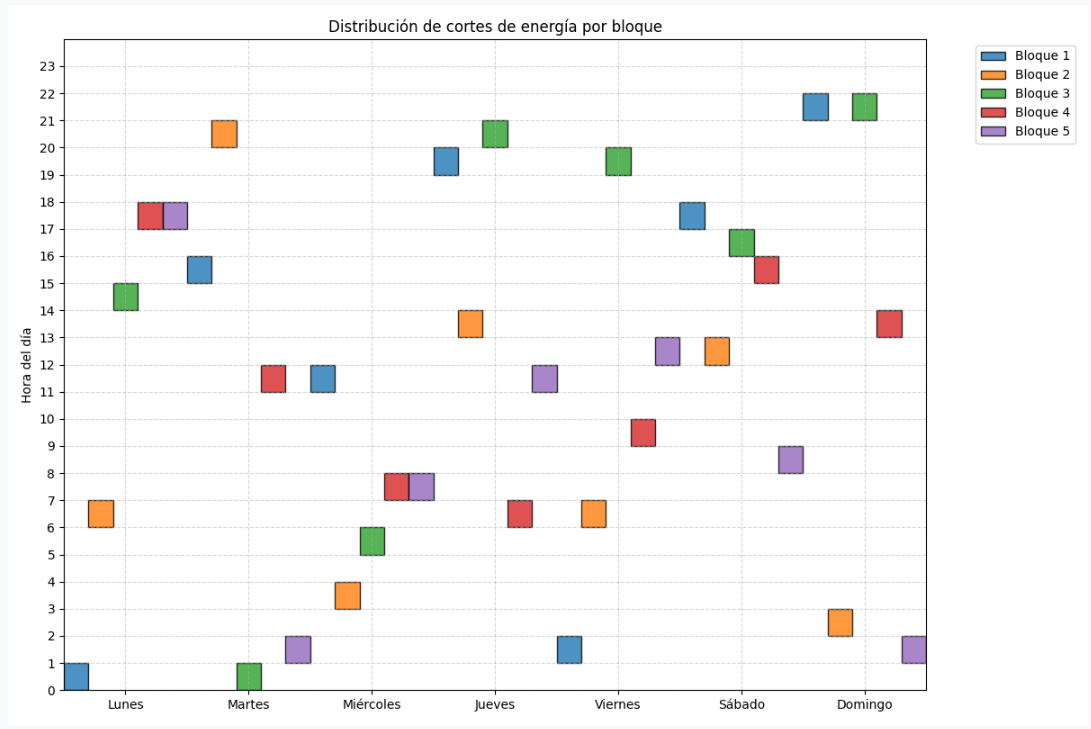
\includegraphics[width=0.8\textwidth]{anexos/6.png}
    \caption{Visualización de horarios de corte por bloque - Gráfico}
\end{figure}

\end{document}
